\section {Overview}

\begin{figure}[!t]
  \centering
  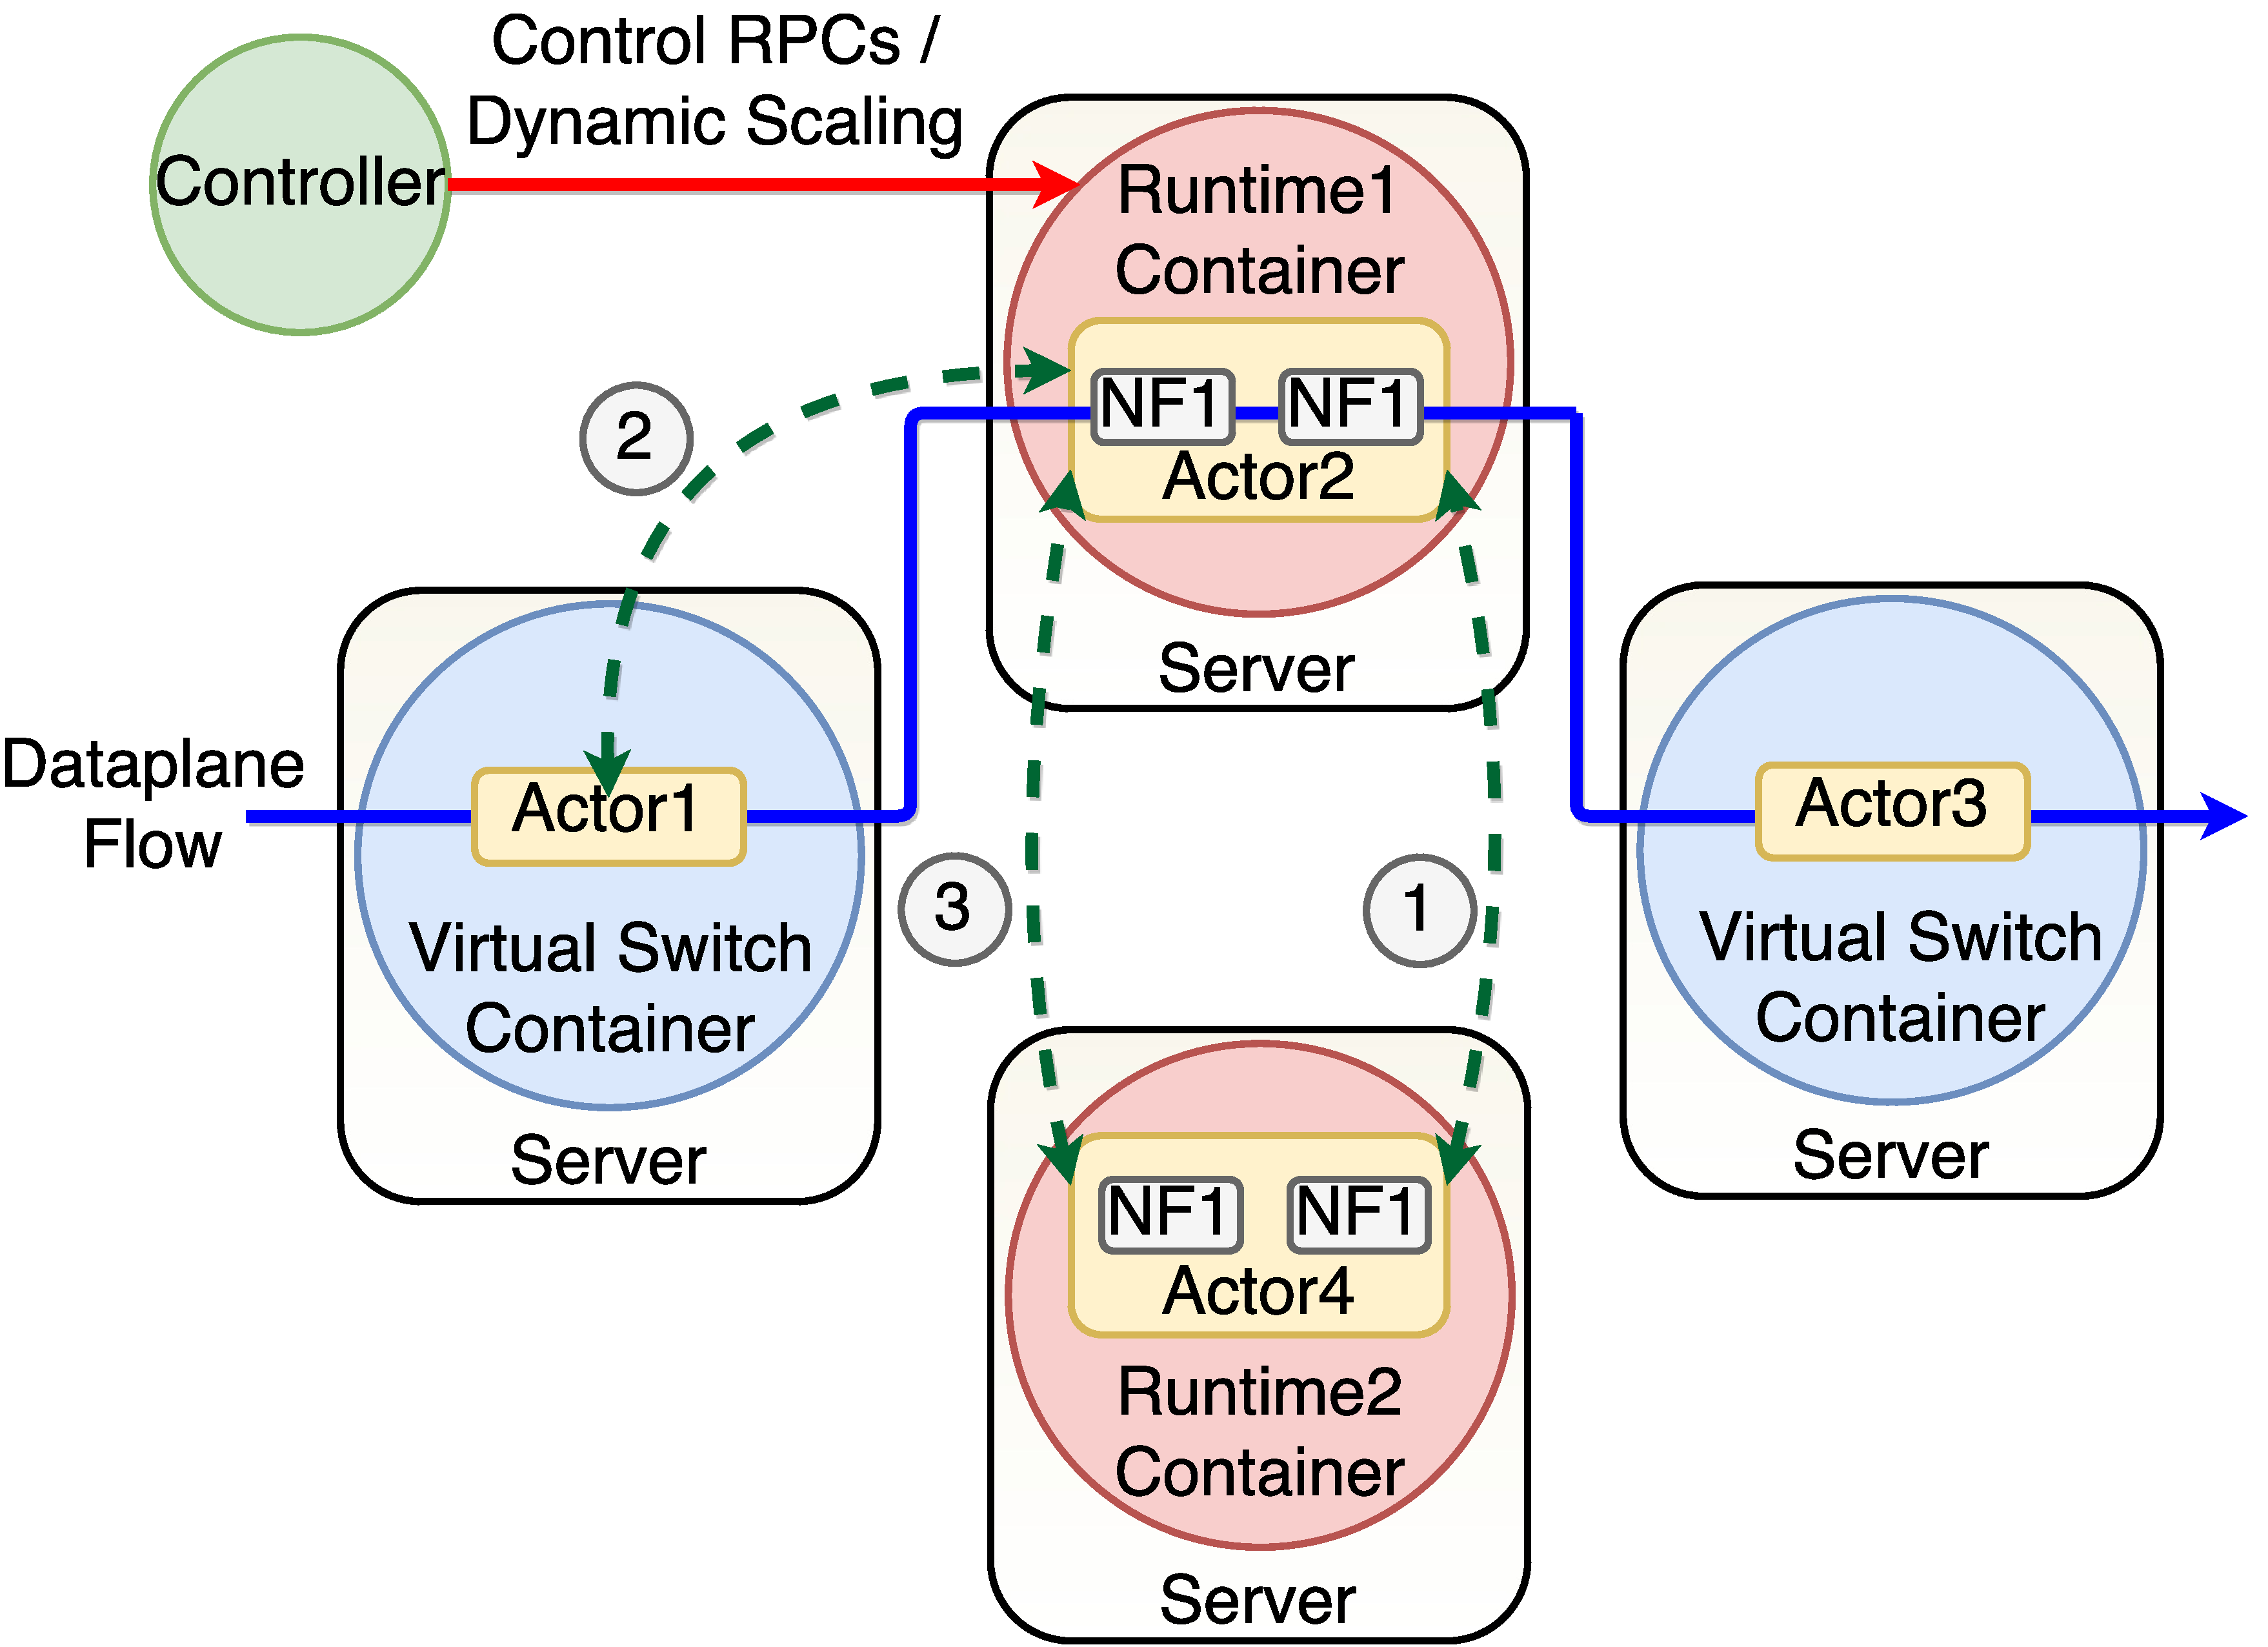
\includegraphics[width=\columnwidth]{figure/final-final-nfactor-cluster.pdf}
  \caption{An overview of NFActor framework.}
  \label{fig:runtime}
\end{figure}

Figure \ref{fig:runtime} demonstrates the basic architecture of NFActor framework, consisting of a light-weight controller, input and output virtual switches and several runtime systems (referred to as \textit{runtime} in short). NFActor framework runs virtual switches and runtimes inside containers, so that they can be quickly rebooted in case of failure and elastically scaled in case of overload.

In NFActor framework, incoming dataplane flows are first sent to the input virtual switch, which dispatches them to runtimes in a round-rubin fashion. The runtime hosts a NF service chain that is determined during runtime initialization and processes incoming flows. When a runtime receives a new flow, it creates a new actor and delegates the packet processing of the flow to that actor. The actor loads all the required NF modules of the service chain when it is created and passes the received flow packet to these NF modules in sequence. Once the service chain processing is finished, the actor sends the packet to an output virtual switch, where the packet is sent to its final destination.

The controller monitors the workload of each runtime and controls dynamic scaling. It also uses control RPCs exposed by the runtime to initiate flow management tasks, including flow migration and replication.
